\documentclass{article}

\usepackage{a4wide}
\usepackage{amsmath}
\usepackage{amssymb}
\usepackage{graphicx}
\usepackage{hyperref}

\newcommand{\Lagr}{\mathcal{L}}

\begin{document}

\title{EM Algorithm}

\author{Valentin Lhermitte}
\date{\today}

\maketitle

\section{Assigment 1 - Estimation of the shape without rotation}

The first assignment was to implement the EM algorithm to estimate the shape s of an object without rotation, 
by finding the maximum likelihood of the parameters $\eta_0$ and $\eta_1$ of the Bernoulli distribution ($\eta_0$ for background and $\eta_1$ for the forground).

The EM algorithm is an iterative algorithm that alternate between the E-step and the M-step.

The goal is to maximize the probability : 

Proof that all we need form the data is the average image $\psi = \frac{1}{m} \sum_{x \in T^m} x$ 
\begin{align*}
    \frac{1}{m} \sum_{x \in T^m}p(x; s, \eta) -> \max_{s, \eta} \tag{1}
\end{align*}

\begin{align*}
    \log p(x; s, \eta) &= \langle x, \eta(s) \rangle - n_{s=0} \log(1 + e^{\eta_0}) - n_{s=1} \log(1 + e^{\eta_1}) \tag{2}
\end{align*}

Subsituting (2) in (1) :
\begin{align*}  
    \frac{1}{m} \sum_{x \in T^m}(\langle x, \eta(s) \rangle - n_{s=0} \log(1 + e^{\eta_0}) - n_{s=1} \log(1 + e^{\eta_1})) \\
    = \langle\psi, \eta(s)\rangle - n_{s=0} \log(1 + e^{\eta_0}) - n_{s=1} \log(1 + e^{\eta_1}) \tag{3}
\end{align*}

\subsection*{E-step}

In the E-step, we compute the posterior probability of the hidden variable $s$ given the data $\psi$ and the current estimate of the parameters $\eta$.
To begin, we set the initial value of the $\eta$ : $\eta_0 = 0$ $\eta_1 = 1$.
We return the estimated value of the hidden variable $s$ and move on with the M-step.

\subsection*{M-step}
In this step, we compute the new estimate of the parameters $\eta$ given the data $\psi$ and the current estimate of the hidden variable $s$.

\begin{align*}
    \eta_0 &= \frac{1}{n_0} \sum_{} \psi (1 - s) \\
    \eta_1 &= \frac{1}{n_1} \sum_{} \psi s
\end{align*}
Where $n_0$ is the number of pixels in the background and $n_1$ is the number of pixels in the foreground. \\
We return the new estimate of the parameters $\eta$ and move on with the E-step.
\newpage

\subsection*{Results}
The algorithm converge and find the right shape of the object (fig. \ref{fig:shape1}) with $\eta_0 = 0.5673$ and $\eta_1 = 0.3436$.

\begin{figure}[h]
    \centering
    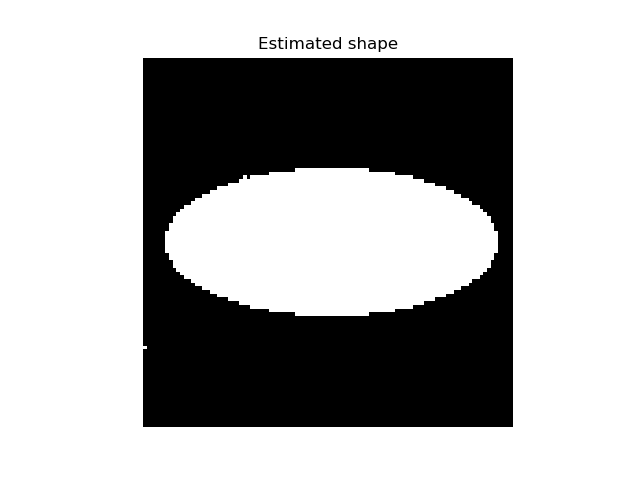
\includegraphics[width=0.6\textwidth]{images/shape1.png}
    \caption{Shape of assignment 1}
    \label{fig:shape1}
\end{figure}


\section{Assigment 2 - Estimation of the shape with rotation}

The second assignment was to implement the EM algorithm to estimate the shape s of an object with rotation.
There would be 4 possible rotation : 0, 90, 180 and 270 degrees.

Again, we will use the EM algorithm to estimate the shape of the object and the rotation.

\subsection*{E-step}
The probability of $\alpha_x(r) = p(r|x;s,\eta)$ \\
The posterior probabilities of $\alpha_x(r)$ can be computed by softmax function:

\begin{align*}
    \alpha_x(r) = softmax_r(\langle x, \eta(T_r s) \rangle + log \pi_r)
\end{align*}

Proof :
\begin{align*}
    \alpha_x(r) &= \frac{p(x|r;s,\eta) p(r)}{\sum p(r|x;s,\eta) p(r)} \\
                &= \frac{e^{\langle x, \eta(T_r s) \rangle - n_{s=0} \log(1 + e^{\eta_0}) - n_{s=1} \log(1 + e^{\eta_1})} \pi_r}{\sum e^{\langle x, \eta(T_r s) \rangle - n_{s=0} \log(1 + e^{\eta_0}) - n_{s=1} \log(1 + e^{\eta_1}) \pi_r}} \\
                &= \frac{e^{\langle x, \eta(T_r s) \rangle + \log \pi_r} e^{- n_{s=0} \log(1 + e^{\eta_0}) - n_{s=1} \log(1 + e^{\eta_1})}}{\sum e^{\langle x, \eta(T_r s) \rangle + log \pi_r} e^{- n_{s=0} \log(1 + e^{\eta_0}) - n_{s=1} \log(1 + e^{\eta_1})}} \\
                &= \frac{e^{\langle x, \eta(T_r s) \rangle + \log \pi_r}}{\sum e^{\langle x, \eta(T_r s) \rangle + \log \pi_r}} \\
                &= softmax_r(\langle x, \eta(T_r s) \rangle + \log \pi_r) \\
\end{align*}

\subsection*{M-step}

In this step, we compute the new estimate of the parameters $\eta$ and $\pi$ given the data $\psi$ and the current estimate of the hidden variable $s$ and $r$.

The maximiser for the pose probabilities $\pi_r$ can be found in closed form using the Lagrange multiplier method:

Lagrangian :
\begin{align*}
    \Lagr = \frac{1}{m} \sum_{x \in T^m} \sum_{r \in R} \alpha_x (r) + \lambda \left( \sum_{r \in R} \pi_r - 1 \right)
\end{align*}

We take the derivative of the Lagrangian with respect to $\pi_r$ and $\lambda$ and set them to zero.
\begin{align*}
    \frac{\partial \Lagr}{\partial \pi_r} = \frac{1}{m} \sum_{x \in T^m} \frac{\alpha_x (r)}{\pi_r} - \lambda = 0
\end{align*}

\begin{align*}
    \frac{\partial \Lagr}{\partial \lambda} = \sum_{r \in R} \pi_r - 1 = 0
\end{align*}


If we solve the equations above, we get :
\begin{align*}
    \pi_r = \frac{1}{m} \sum_{x \in T^m} \alpha_x (r)
\end{align*}

\begin{align*}
    \lambda = \sum_{r \in R} \alpha_x (r) = 1
\end{align*}

Now we can fix $\pi_r$ and maximize the parameters $\eta$ and the shape $s$, by using the same method as in the first assignment, using $shape\_mle()$.

Proof that all you need from the data is the array : 
\begin{align*}
    \psi = \frac{1}{m} \sum_{x \in T^m} \sum_{r \in R} \alpha_x (r) T_r^T x
\end{align*}

\begin{align*}
    \frac{1}{m} \sum_{x \in T^m} \sum_{r} \alpha_x (r) (\langle T_r^T x, \eta(s) \rangle - n_{s=0} \log(1 + e^{\eta_0}) - n_{s=1} \log(1 + e^{\eta_1})) \\
    = \left\langle \frac{1}{m} \sum_{x \in T^m} \sum_{r}  \alpha_x (r) T_r^T x, \eta(s) \right\rangle - n_{s=0} \log(1 + e^{\eta_0}) - n_{s=1} \log(1 + e^{\eta_1}) \\
    = \langle \psi, \eta(s) \rangle - n_{s=0} \log(1 + e^{\eta_0}) - n_{s=1} \log(1 + e^{\eta_1})
\end{align*}

\newpage
\subsection*{Results}
The algorithm converge and find the right shape of the object (fig. \ref{fig:shape2}) with $\eta$ = [0.4516, 0.5502] and $\pi$ = [0.3 0.3 0.2 0.2].

\begin{figure}[h]
    \centering
    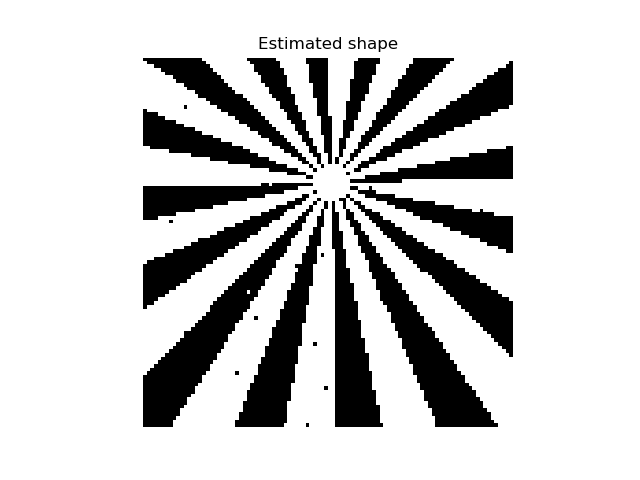
\includegraphics[width=0.6\textwidth]{images/shape2.png}
    \caption{Shape of assignment 2}
    \label{fig:shape2}
\end{figure}


\end{document}